\section{Material and methods}\label{material-and-methods}

In this section, we present in more details, the datasets and the
methodology we used. All analyses have been performed using R
environment software (table S1 includes functions and packages we used).

\subsection{Datasets}\label{datasets}

Sites for the five datasets are reported on five maps gathered in Fig
S1. Below, we describe in more details the five datasets. The total
number of species, the number of species present in at least 1\% of the
total number of site and the number of species for which traits
information were available are reported in table S2.

\subsubsection{Willows leafs network}\label{willows-leafs-network}

\subsubsection{Pitcher plants network}\label{pitcher-plants-network}

\subsubsection{Caribbean Hummingbirds-Plant
network}\label{caribbean-hummingbirds-plant-network}

\subsubsection{North American Trees
datasets}\label{north-american-trees-datasets}

\paragraph{Traits-based distance}\label{traits-based-distance}

We used a distance built upon nine functional traits whose values were
retrieved from ({\textbf{???}}), see \textbf{Supplementary Table 3}
available at
\url{http://onlinelibrary.wiley.com/doi/10.1111/j.1466-8238.2010.00592.x/suppinfo}.
Each of the nine selected variables were centered and scaled (R
functions used reported in table S1) then used as is to derive Euclidean
distances for all pairs of species. Then, we use agglomeration
clustering with Ward's method (implemented in the \emph{hclust()}
function we used, see Table S1) to obtain the dendrogram presented in
\ref{fig:dendro}.

\subsubsection{French Breeding Birds Survey
datasets}\label{french-breeding-birds-survey-datasets}

\paragraph{Traits-based distance}\label{traits-based-distance-1}

We used 73 traits that are boolean variable (see Table S4) we kept as is
to derive Euclidean distances for all pairs of species.

\subsection{Building metawebs}\label{building-metawebs}

For four datasets, we built network based on all observed interactions
and derived associated quantities, \emph{i.e.} the connectance of the
metawebs, the degrees of species and the shortest-path, using the R
package ``igraph'' (table S1).

\subsection{Co-occurrence measurement}\label{co-occurrence-measurement}

For a given pair of species \(i\) and \(j\), we examined the
relationship between the observed co-occurrence \(O_{i,j}\) and the
expected co-occurrence \(E_{i,j}\). Here, we provide more information
about the three methods wed used to analyse co-occurrence.

\subsection{Hypergeometric
distribution}\label{hypergeometric-distribution}

This distribution has been mentioned in a different context (see
{\textbf{???}}) and have been fully exploited in ({\textbf{???}})
despite the author never mentioned it is a classical distribution. To
clarify this, we start from the distribution written in equation (1) in
Veech (2013). We consider the co-occurrence of two species on \(n\)
sites. Species 1 is present in \(n_1\) while species 2 is present in
\(n_2\) sites. The probability of having \(j\) co\_occurrence, \(p_j\)
is:

\[ p_j= \frac{\binom{n}{j} \binom{n-j}{n_2-j} \binom{n-n_2}{n_1-j}}{\binom{n}{n_2} \binom{n}{n_2}} \]

if \(\max{0, n_1+n_2-n} \leq j \leq \min{n_1, n_2}\) and 0 otherwise.
The expression above yields:

\[ p_j= \frac{n!}{(n-j)!j!} \frac{(n-j)!}{(n-j-n_2+j)!(n_2-j)!} \frac{(n-n_2)!}{(n-n_2-n_1+j)!(n_1-j)!} \frac{(n-n_1)!n_1!}{n!} \frac{1}{\binom{n}{n_2}} \]

by rearrangement:

\[ p_j= \frac{1}{j!} \frac{1}{(n_2-j)!} \frac{1}{(n-n_2-n_1+j)!(n_1-j)!} \frac{(n-n_1)!n_1!}{1} \frac{1}{\binom{n}{n_2}} \]

once sorted out, this results in:

\[ p_j= \frac{\binom{n_1}{j} \binom{n-n_1}{n_2-j}}{\binom{n}{n_2}} \]

Thus, the number of co-occurrence follows a hypergeometric distribution
of parameters \((n,n_1,n_2)\) we used to calculated the expected
co-occurrence \(E_{i,j}\) under the hypothesis that all site were
identical for all species.

\subsection{GLM and RF}\label{glm-and-rf}

For GLM and RF, \(E_{i,j}\) correspond to probabilities of occurrence
computed based on climatic data. R functions are reported in Table S1.

\subsubsection{Climatic data}\label{climatic-data}

We used the global climate layers provided data WolrdClim, version 1.4,
available at \url{http://www.worldclim.org} ({\textbf{???}}). For each
dataset, we performed a principal component analysis and keep as many
axes as needed to explain 90\% of the total inertia. We used these axis
in GLM and RF.

\subsubsection{Generalized Linear Model}\label{generalized-linear-model}

For all datasets, we performed a Generalized Linear Model
({\textbf{???}}) using all the axis provided by the PCA as polynomials
of degree 2. To constraints the number of parameters, we did not
evaluate the interactions among axis. We also performed a selection
model based on the Akaike's information criterion (AIC) C in a Stepwise
Algorithm. R functions used to carry out the analyses are indexed in
table SX.

\subsubsection{Random Forests}\label{random-forests}

Random Forests ({\textbf{???}}) were performed using the same formula as
for GLMs. For all species, 10000 trees were computed and the probability
for a species being in a given site were calculated based on the number
of votes the sites were granted.

\subsubsection{Evaluating the models}\label{evaluating-the-models}

For all species, we assess the performance of the Species Distribution
Models we used, \emph{i.e.} Generalized Linear Model and Random Forest,
using the Area Under the Receiver Operating Characteristic (AUROC)
({\textbf{???}}). We present the results as a cumulative sum of
frequencies corresponding to the score for all species for each of the
four ecological systems we studied (see Fig ({\textbf{???}})).

\section{Supporting Tables}\label{supporting-tables}

\subsubsection{R packages used}\label{r-packages-used}

\begin{longtable}[]{@{}lrrrr@{}}
\toprule
Analysis & Function & Package name & Version & Citation\tabularnewline
\midrule
\endhead
Scaling and Centering & scale & base & 3.3.1 & R Core Team
(2015)\tabularnewline
Euclidean distance & dist & stats & 3.3.1 & R Core Team
(2015)\tabularnewline
Clustering & hclust & stats & 3.3.1 & R Core Team (2015)\tabularnewline
PCA & dudi.pca & ade4 & 1.7.4 & Dray and Dufour (2007)\tabularnewline
GLM & glm & stats & 3.3.1 & R Core Team (2015)\tabularnewline
GLM Selection & step & stats & 3.3.1 & R Core Team (2015)\tabularnewline
Degree of species & degree & igraph & 1.0.1 &
({\textbf{???}})\tabularnewline
Shortest Paths & shortest.paths & igraph & 1.0.1 &
({\textbf{???}})\tabularnewline
AUROC & somers2 & Hmisc & 3.17.2 & ({\textbf{???}})\tabularnewline
TSN retrieving & get\_tsn & taxize & 0.7.4 & ({\textbf{???}}),
({\textbf{???}})\tabularnewline
Wilcoxon tests & wilcox.test & stats & 3.3.1 & R Core Team
(2015)\tabularnewline
\bottomrule
\end{longtable}

\textbf{Supplementary Table 1}: R and packages used for the analyses.
GLM: Generalized Linear Model, PCA: Principal Component Analysis. AUROC:
Area Under the Receiver Operating Characteristic.\{\#tbl:code\}

\begin{longtable}[]{@{}lrrr@{}}
\toprule
Type & Total & Selected & Traits\tabularnewline
\midrule
\endhead
Willow Leaf Network & 274 & 156 & - ~\tabularnewline
Pitcher Plants Network & 91 & 53 & -\tabularnewline
Caribbean Hummingbirds Network & 62 & 62 & -\tabularnewline
North American Trees & 31 & 31 & 31\tabularnewline
French Breeding Birds Survey & 340 & 179 & 321\tabularnewline
\bottomrule
\end{longtable}

\textbf{Supplementary Table 2}: For each datasets the total number of
species (column \emph{Total}), the number of species present in more
that 1\% of the total number of sites (column \emph{Selected}), andthe
number of species for which traits information are available (column
\emph{Traits}). The symbol `-' means `not relevant'. \{\#tbl:numsp\}

\begin{longtable}[]{@{}lrrrrrrrrrr@{}}
\toprule
Species & TSN & maxH & GR & WD & TolS & TolD & AM & EM & LMA &
Nmass\tabularnewline
\midrule
\endhead
Abies balsamea & 18032 & 25 & 1 & 0.34 & 5.0 & 1.0 & 0 & 1 & 151.00 &
1.66\tabularnewline
Acer negundo & 28749 & 20 & 3 & 0.44 & 3.5 & 3.0 & 1 & 0 & 37.04 &
2.50\tabularnewline
Acer rubrum & 28728 & 25 & 3 & 0.49 & 3.4 & 1.8 & 1 & 0 & 71.09 &
1.91\tabularnewline
Acer saccharum & 28731 & 35 & 1 & 0.56 & 4.8 & 2.3 & 1 & 0 & 70.63 &
1.83\tabularnewline
Betula alleghaniensis & 19481 & 25 & 3 & 0.55 & 3.2 & 3.0 & 0 & 1 &
46.08 & 2.20\tabularnewline
Betula papyrifera & 19489 & 25 & 3 & 0.48 & 1.5 & 2.0 & 0 & 1 & 77.88 &
2.31\tabularnewline
Carpinus caroliniana & 19504 & 8 & 1 & 0.58 & 4.6 & 2.0 & 0 & 1 & 49.05
& 2.15\tabularnewline
Carya cordiformis & 19227 & 25 & 1 & 0.60 & 2.1 & 4.0 & 0 & 1 & 44.05 &
2.60\tabularnewline
Fagus grandifolia & 19462 & 25 & 1 & 0.56 & 4.8 & 1.5 & 0 & 1 & 61.22 &
2.04\tabularnewline
Fraxinus americana & 32931 & 30 & 2 & 0.55 & 2.5 & 2.4 & 1 & 0 & 76.75 &
2.12\tabularnewline
Fraxinus nigra & 32945 & 20 & 2 & 0.45 & 3.0 & 2.0 & 1 & 0 & 71.94 &
2.10\tabularnewline
Fraxinus pennsylvanica & 32929 & 25 & 3 & 0.53 & 3.1 & 3.9 & 1 & 0 &
87.72 & 1.80\tabularnewline
Larix laricina & 183412 & 25 & 3 & 0.48 & 1.0 & 2.0 & 0 & 1 & 120.00 &
1.36\tabularnewline
Ostrya virginiana & 19511 & 12 & 1 & 0.63 & 4.6 & 3.3 & 1 & 0 & 37.04 &
2.20\tabularnewline
Picea glauca & 183295 & 25 & 1 & 0.35 & 4.2 & 2.9 & 0 & 1 & 302.86 &
1.28\tabularnewline
Picea mariana & 183302 & 20 & 1 & 0.41 & 4.1 & 2.0 & 0 & 1 & 294.12 &
1.12\tabularnewline
Picea rubens & 18034 & 25 & 2 & 0.38 & 4.4 & 2.5 & 0 & 1 & 304.67 &
1.15\tabularnewline
Pinus banksiana & 183319 & 20 & 3 & 0.42 & 1.4 & 4.0 & 0 & 1 & 243.90 &
1.24\tabularnewline
Pinus resinosa & 183375 & 25 & 3 & 0.39 & 1.9 & 3.0 & 0 & 1 & 294.12 &
1.17\tabularnewline
Pinus strobus & 183385 & 30 & 3 & 0.36 & 3.2 & 2.3 & 0 & 1 & 121.92 &
1.42\tabularnewline
Populus balsamifera & 22453 & 25 & 3 & 0.37 & 1.3 & 1.8 & 1 & 1 & 83.46
& 1.95\tabularnewline
Populus grandidentata & 22463 & 20 & 3 & 0.39 & 1.2 & 2.5 & 1 & 1 &
70.45 & 2.50\tabularnewline
Populus tremuloides & 195773 & 25 & 3 & 0.37 & 1.2 & 1.8 & 1 & 1 & 82.02
& 2.16\tabularnewline
Prunus pensylvanica & 24799 & 12 & 3 & 0.36 & 1.0 & 2.0 & 1 & 1 & 50.00
& 2.40\tabularnewline
Quercus alba & 19290 & 35 & 1 & 0.60 & 2.9 & 3.6 & 0 & 1 & 81.21 &
2.39\tabularnewline
Quercus macrocarpa & 19287 & 15 & 1 & 0.58 & 2.7 & 3.9 & 0 & 1 & 92.74 &
2.27\tabularnewline
Quercus rubra & 19408 & 25 & 2 & 0.56 & 2.8 & 2.9 & 0 & 1 & 84.20 &
2.06\tabularnewline
Thuja occidentalis & 505490 & 15 & 1 & 0.30 & 3.5 & 2.7 & 1 & 0 & 223.00
& 1.02\tabularnewline
Tsuga canadensis & 183397 & 30 & 1 & 0.40 & 4.8 & 1.0 & 0 & 1 & 122.55 &
0.99\tabularnewline
Ulmus americana & 19049 & 35 & 3 & 0.46 & 3.1 & 2.9 & 1 & 0 & 79.47 &
2.07\tabularnewline
Ulmus rubra & 19050 & 25 & 3 & 0.48 & 3.3 & 3.0 & 1 & 0 & 59.88 &
2.50\tabularnewline
\bottomrule
\end{longtable}

\textbf{Supplementary Table 3}: Tree species and traits used.
Abbreviations are as follows: TSN - Taxonomic Serial Number defined by
Integrated Taxonomic Information System (ITIS), maxH - Average maximum
height, GR - Growth rate, WD - Wood Density, TolS - Shade tolerance,
TolD - Drought tolerance, AM - Arbuscular mycorrhiza (Endomycorrhiza),
EM - Ectomycorrhiza, LMA - Leaf mass per area, Nmass - Nitrogen content
per leaf mass unit({\textbf{???}}) availale at
\url{http://onlinelibrary.wiley.com/doi/10.1111/j.1466-8238.2010.00592.x/suppinfo}.\{\#tbl:trees\}

\begin{longtable}[]{@{}lr@{}}
\toprule
Category & Trait name\tabularnewline
\midrule
\endhead
Activity & Nocturnal\tabularnewline
Activity & Crepuscular\tabularnewline
Activity & Diurnal\tabularnewline
Diet & Seeds, nuts or grain\tabularnewline
Diet & Fruits / frugivory\tabularnewline
Diet & Vegetative\tabularnewline
Diet & invert\tabularnewline
Diet & fish\tabularnewline
Diet & Very small mammals\tabularnewline
Diet & Large mammals\tabularnewline
Diet & Herptile\tabularnewline
Diet & Small birds\tabularnewline
Diet & Long birds\tabularnewline
Diet & Vertebrate\tabularnewline
Diet & Bones\tabularnewline
Diet & Carrion\tabularnewline
Feeding behavior & Pursuit (air and/or aquatic)\tabularnewline
Feeding behavior & Sally\tabularnewline
Feeding behavior & Foliage gleaning\tabularnewline
Feeding behavior & Pouncing\tabularnewline
Feeding behavior & Grazing\tabularnewline
Feeding behavior & Picking, pecking or stabbing\tabularnewline
Feeding behavior & Digging\tabularnewline
Feeding behavior & Overturning\tabularnewline
Feeding behavior & Probing\tabularnewline
Feeding behavior & Filtering\tabularnewline
Feeding habitat & Water-surface\tabularnewline
Feeding habitat & Underwater\tabularnewline
Feeding habitat & Water\tabularnewline
Feeding habitat & Mud\tabularnewline
Feeding habitat & Ground\tabularnewline
Feeding habitat & Canopy\tabularnewline
Feeding habitat & Shrub (low and high)\tabularnewline
Feeding habitat & Vegetation\tabularnewline
Feeding habitat & Air\tabularnewline
Foraging habitat & Wet grassland, meadows, fens, sedges or
tundra\tabularnewline
Foraging habitat & Dry grassland\tabularnewline
Foraging habitat & Rocky slope\tabularnewline
Foraging habitat & Fast river/stream\tabularnewline
Foraging habitat & Slow river/stream\tabularnewline
Foraging habitat & Shore (marine)\tabularnewline
Foraging habitat & Salt marsh\tabularnewline
Foraging habitat & Mud or silt\tabularnewline
Foraging habitat & Sandy gravel/beach\tabularnewline
Foraging habitat & Reed marshes\tabularnewline
Foraging habitat & Conifer\tabularnewline
Foraging habitat & Mixed forest\tabularnewline
Foraging habitat & Deciduous\tabularnewline
Foraging habitat & Mediterranean oak or other\tabularnewline
Foraging habitat & Open/low forest\tabularnewline
Foraging habitat & Forest or habitat edge\tabularnewline
Foraging habitat & Shrub/bush\tabularnewline
Foraging habitat & Urban\tabularnewline
Foraging habitat & Garden\tabularnewline
Foraging habitat & High air\tabularnewline
Nesting habitat & Wet grassland, meadows, fens, sedges or
tundra\tabularnewline
Nesting habitat & Dry grassland\tabularnewline
Nesting habitat & Banks/sand/mud\tabularnewline
Nesting habitat & Rock surface/outcrops\tabularnewline
Nesting habitat & Near water/shore/island\tabularnewline
Nesting habitat & Sand gravel/beach\tabularnewline
Nesting habitat & Reed marshes\tabularnewline
Nesting habitat & Conifer\tabularnewline
Nesting habitat & Mixed forest\tabularnewline
Nesting habitat & Deciduous\tabularnewline
Nesting habitat & Mediterranean oak and other\tabularnewline
Nesting habitat & Open/low forest\tabularnewline
Nesting habitat & Shrub/bush\tabularnewline
Nesting habitat & Urban\tabularnewline
Nesting habitat & Garden\tabularnewline
Nesting location & Elevated\tabularnewline
Nesting location & Tree hole\tabularnewline
Nesting location & Ground\tabularnewline
\bottomrule
\end{longtable}

\textbf{Supplementary Table 4}: List of the Boolean traits used to
derive Euclidean distances between all pairs of species in the French
Breeding Birds Survey.

\newpage

\section{Supporting Figures}\label{supporting-figures}

\begin{figure}[htbp]
\centering
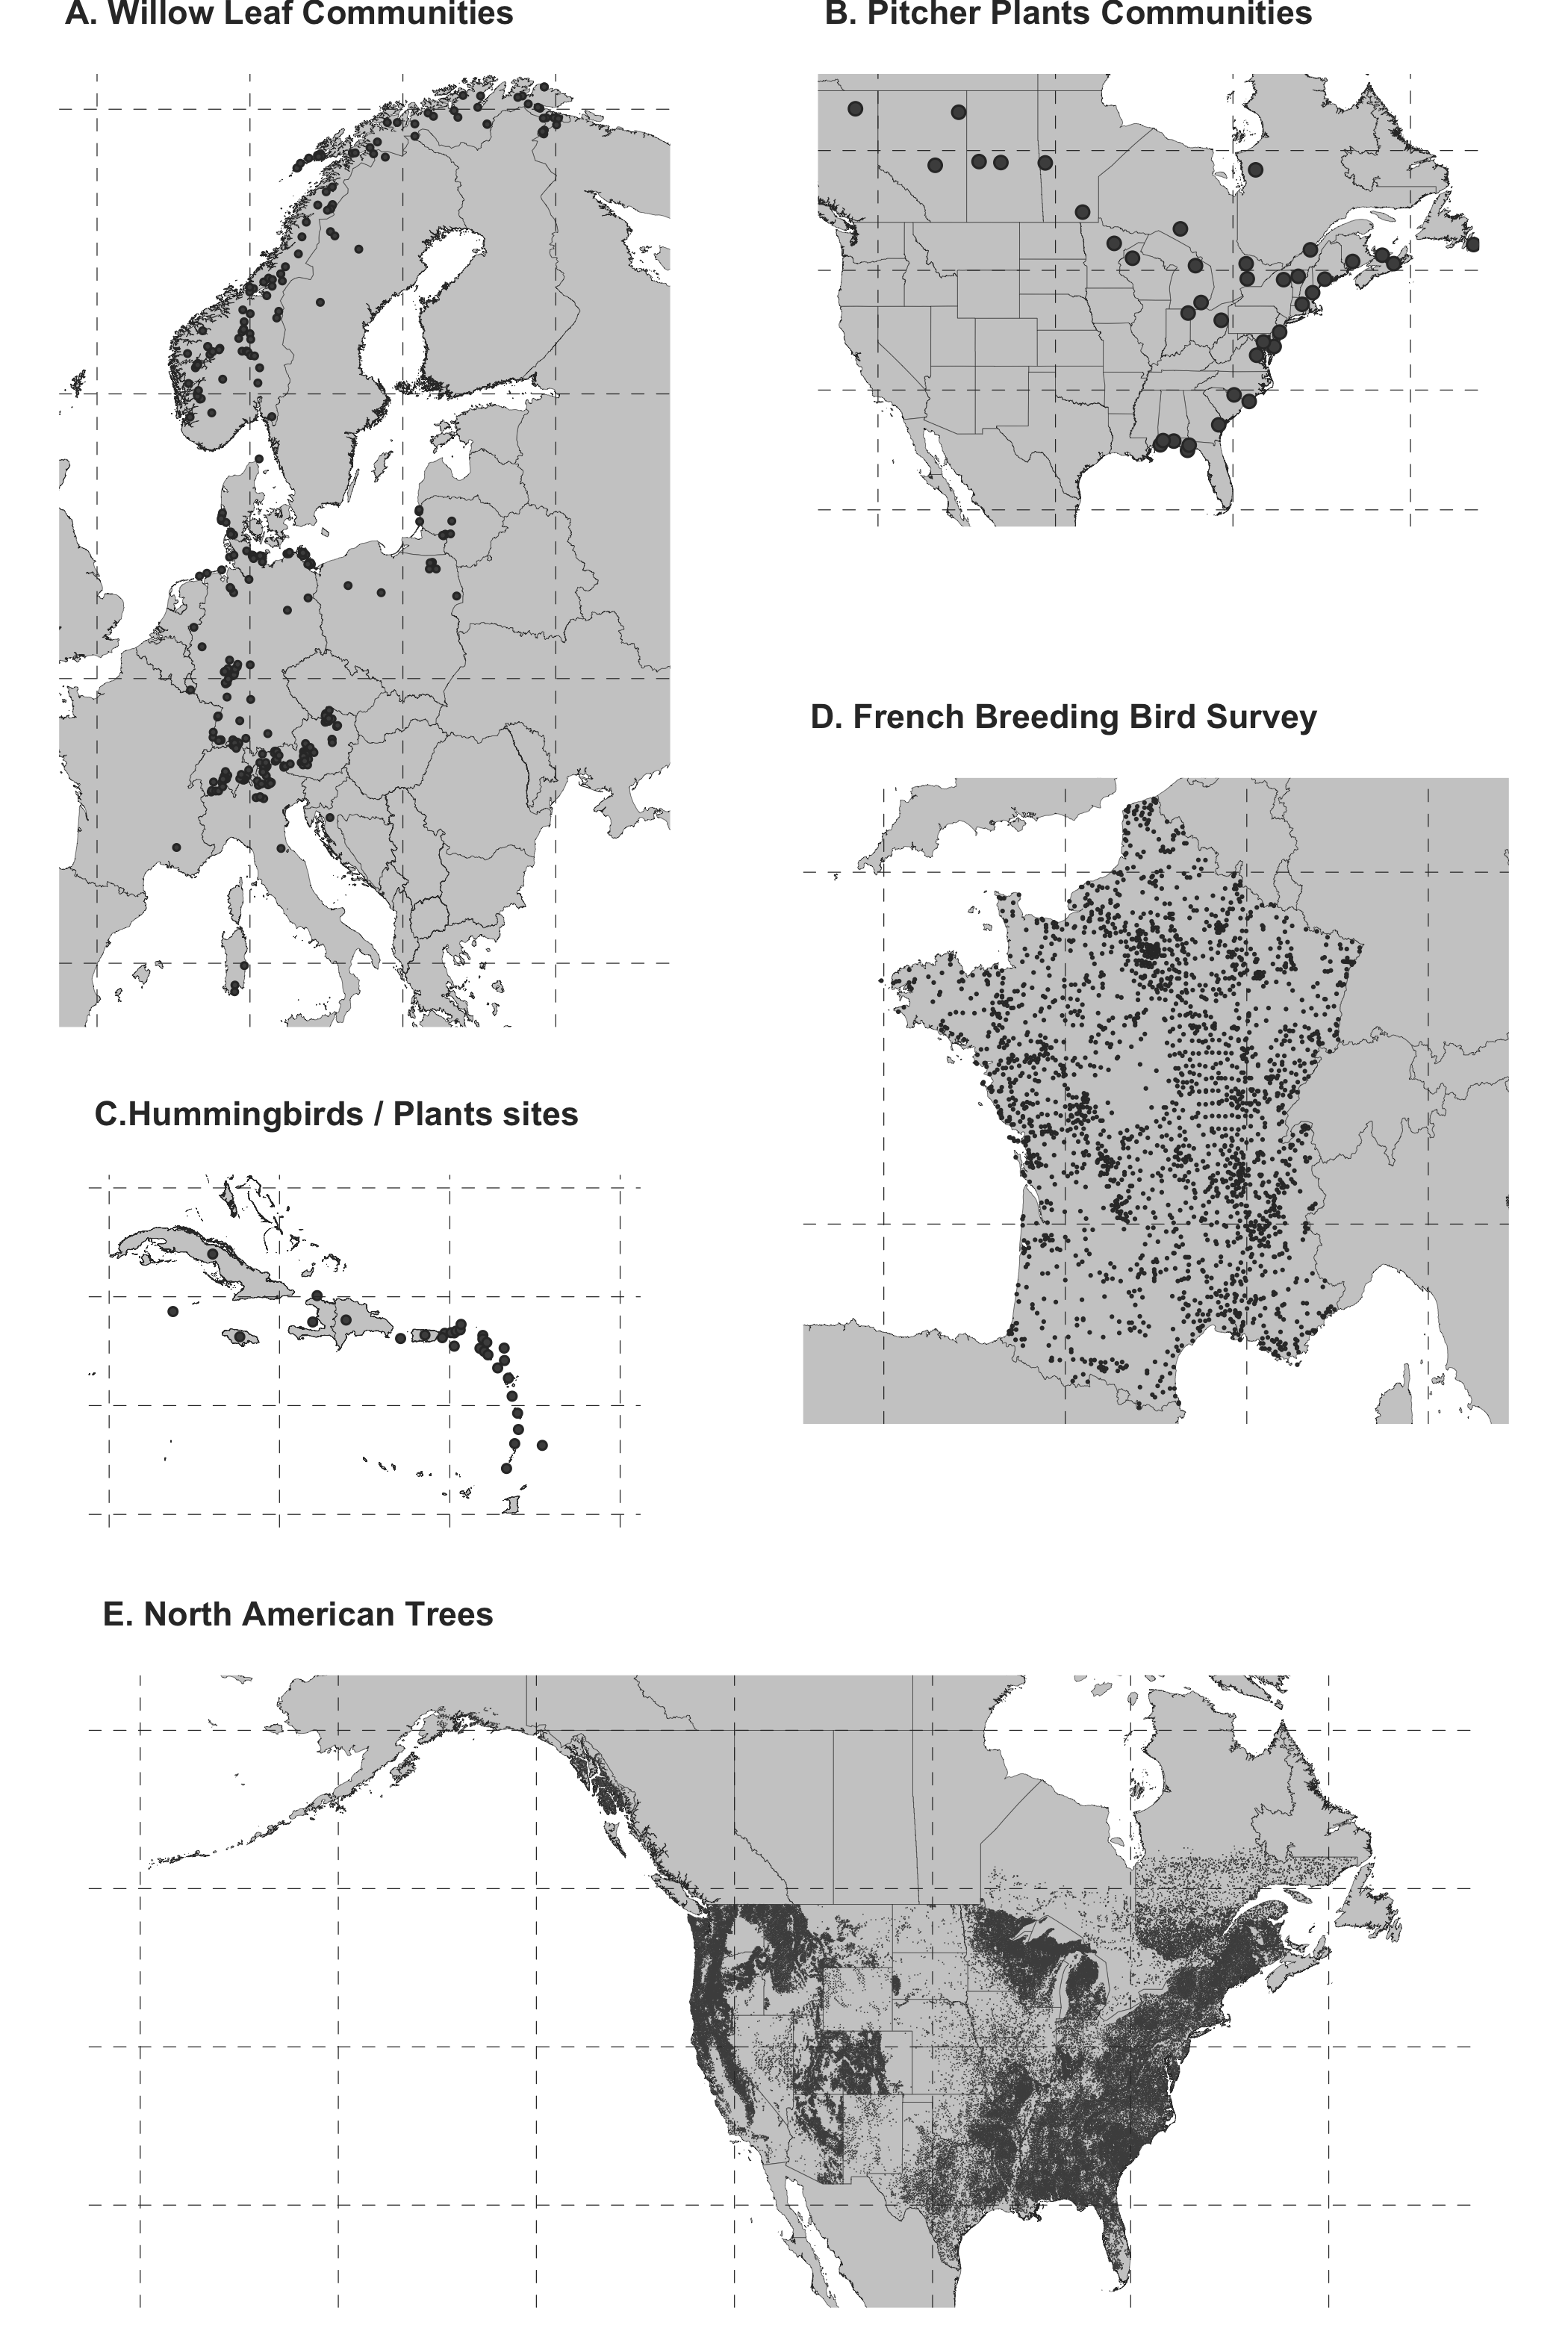
\includegraphics{../fig/figS1.png}
\caption{\textbf{Sites of the study}\label{fig:maps}}
\end{figure}

\newpage

\begin{figure}[htbp]
\centering
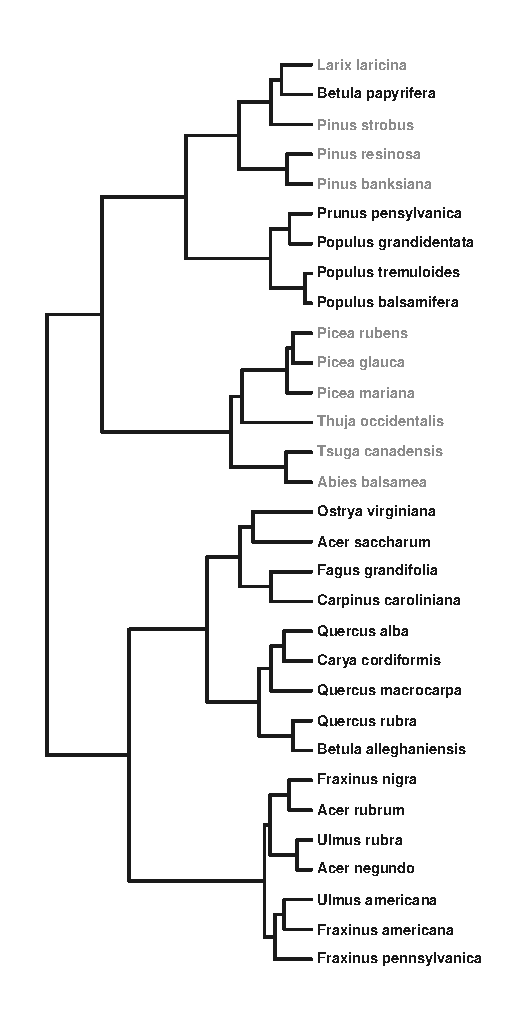
\includegraphics{../fig/figS2.pdf}
\caption{\textbf{Dendrogram representing the trait-based distances
between the 31 species studied in the North American tree datasets.}
Names of angiosperm species are written in dark grey while names of
Gymnosperm species are in a lighter grey.\label{fig:dendro}}
\end{figure}

\newpage

\begin{figure}[htbp]
\centering
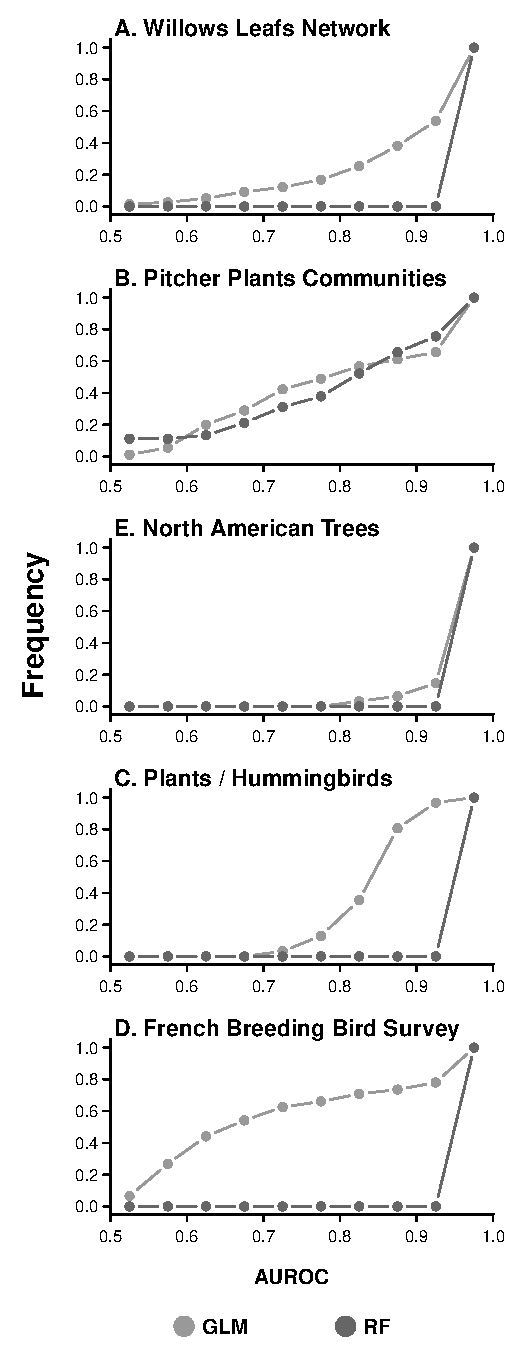
\includegraphics{../fig/figS3.pdf}
\caption{\textbf{Evaluation of the SDM approaches} For each dataset, the
distributions of performance of generalized linear models (light grey
symbols) and random Forest (dark grey symbols) for all species are
presented.\label{fig:auc}}
\end{figure}

\newpage

\begin{figure}[htbp]
\centering
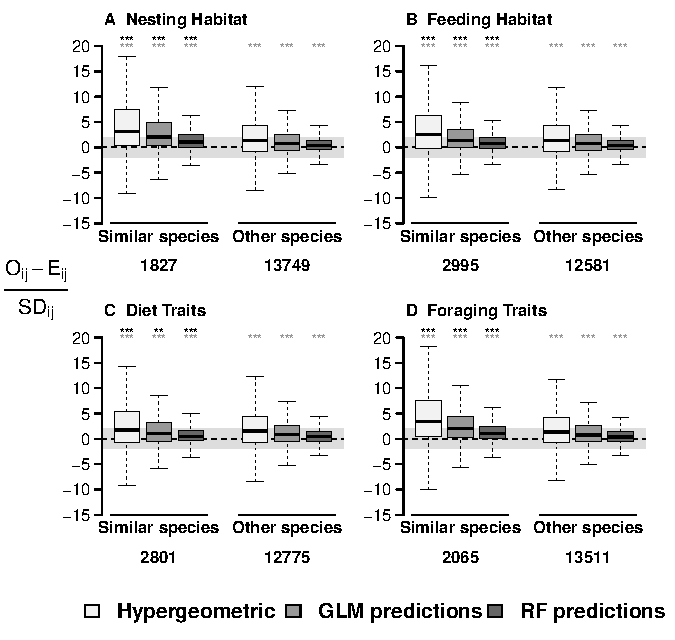
\includegraphics{../fig/figS4.pdf}
\caption{** Co-occurrence and the nature of the trait-based distance in
the FBBS dataset** The different panels correspond to four different set
of trait upon which for different distance are built. Similar species
are defined as the species for which the trait-based distance is less
than or equal to the lower decile of this distance distribution. Note
that outliers are not displayed. The light grey rectangle corresponds to
the 95\% confidence interval for the standard normal distribution which
gives insight into the proportion of pairs of species significantly
different from 0. P values were computed using the Wilcoxon rank sum
test, to compare interacting versus not-interacting Z-score distribution
calculated for the three different methods (black symbols) and to show
whether whether Z-score were greater for hypergeometric versus GLM and
whether GLM versus RF (grey symbols).}\label{figdist}
\end{figure}

\newpage

\begin{figure}[htbp]
\centering
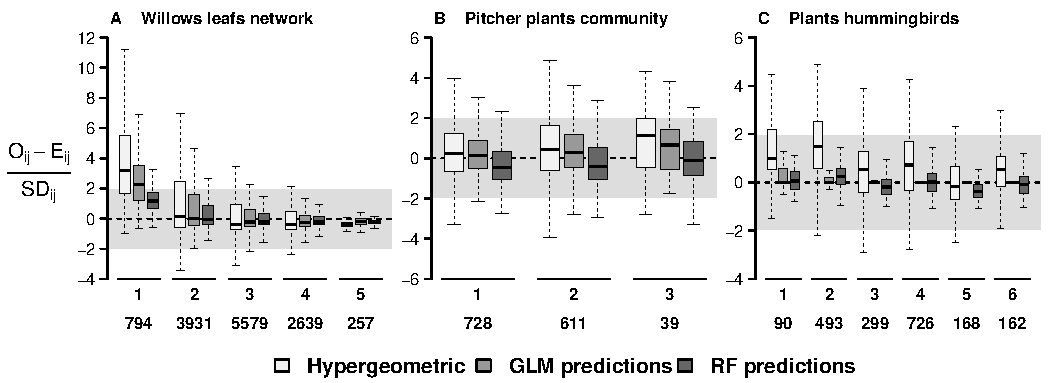
\includegraphics{../fig/figS5.pdf}
\caption{\textbf{Co-occurrence signal decays when the shortest path
between a pair of species decay} Distribution of Z-scores for all
interactions are grouped by shortest-path indicated by the first numbers
below boxplots. The other figures below stand for the number of pairs of
species included within the distributions.\label{fig:sht_pth2}}
\end{figure}

\newpage

\begin{figure}[htbp]
\centering
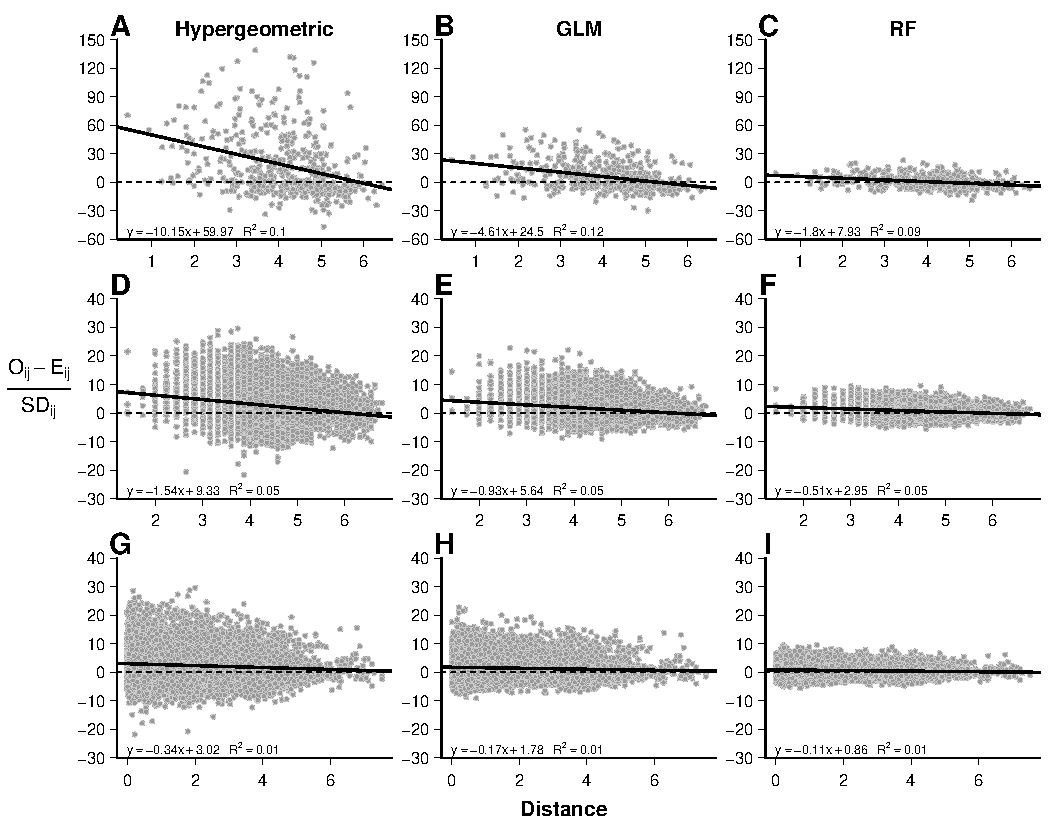
\includegraphics{../fig/figS6.pdf}
\caption{\emph{Changes co-occurrence signal when increasing the distance
between two species} Points represent the result for all pairs of
interaction for two datasets: the North American Tree dataset (A=C) and
the FBBS (D-I). For the latter, we used the trait-based distance
computed with all available traits (D-F) and the body-size ratios (the
lighter species over the heavier, panels G-I). In each panel, the
equation on the bottom-left corner indicated the results of the linear
regression depicted by the dotted line.\label{fig:distrev}}
\end{figure}

\newpage

\begin{figure}[htbp]
\centering
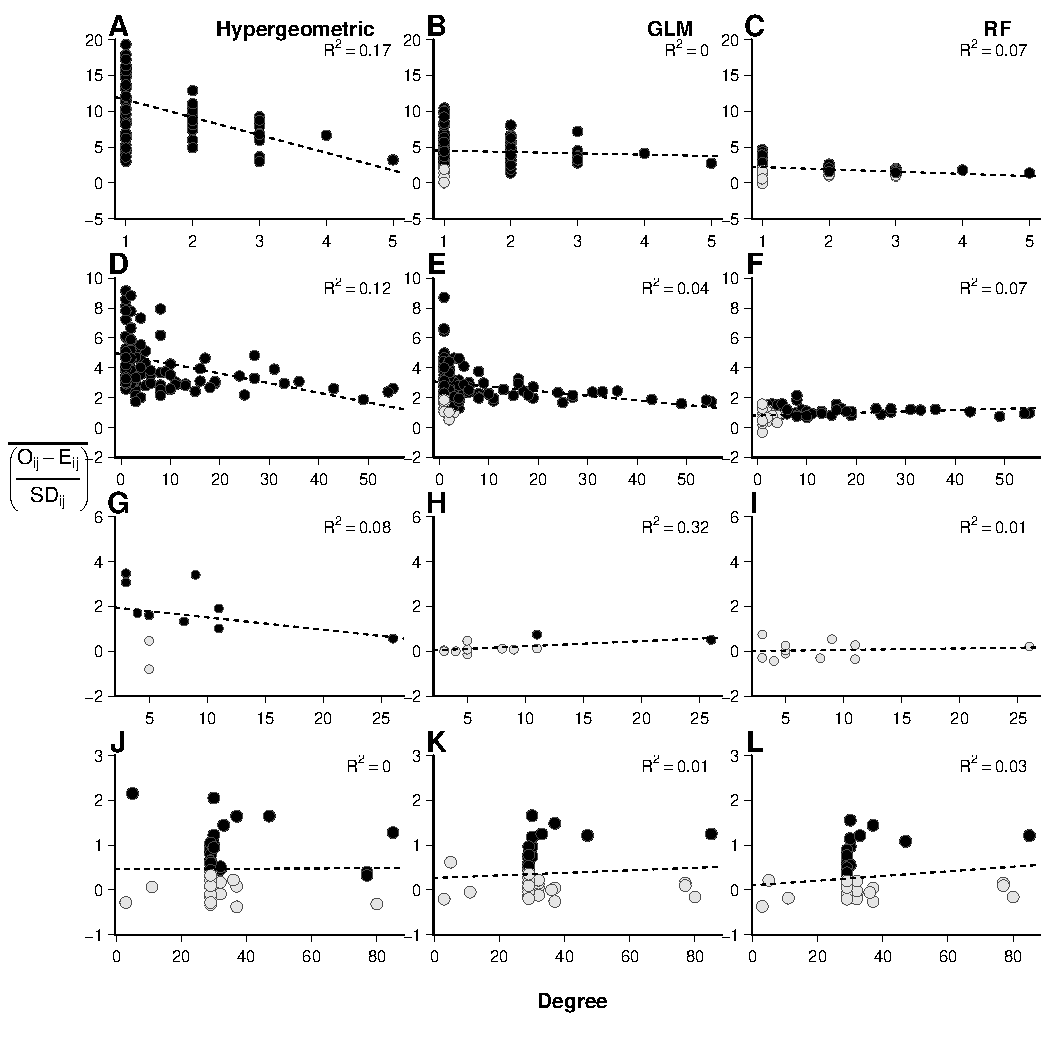
\includegraphics{../fig/figS7.pdf}
\caption{\textbf{The degree of species partially explains the decrease
of the co-occurrence strength} For the herbivores (A-C) and the
parasitoids in the willow leafs network datasets (D-F), the hummingbirds
in the Caribbean hummingbirds datasets (G-I) and all species in the
pitcher plants network that consume other species (J-L) the mean Z-score
is plotted against the degree of the species. Black symbols are mean
Z-scores significantly different from 0 (see SI Text). In each panel,
the dotted line represents the linear regression \(y~ax+b\) for which
the \(R^2\) is provided.\label{fig:degree}}
\end{figure}

\newpage

\begin{figure}[htbp]
\centering
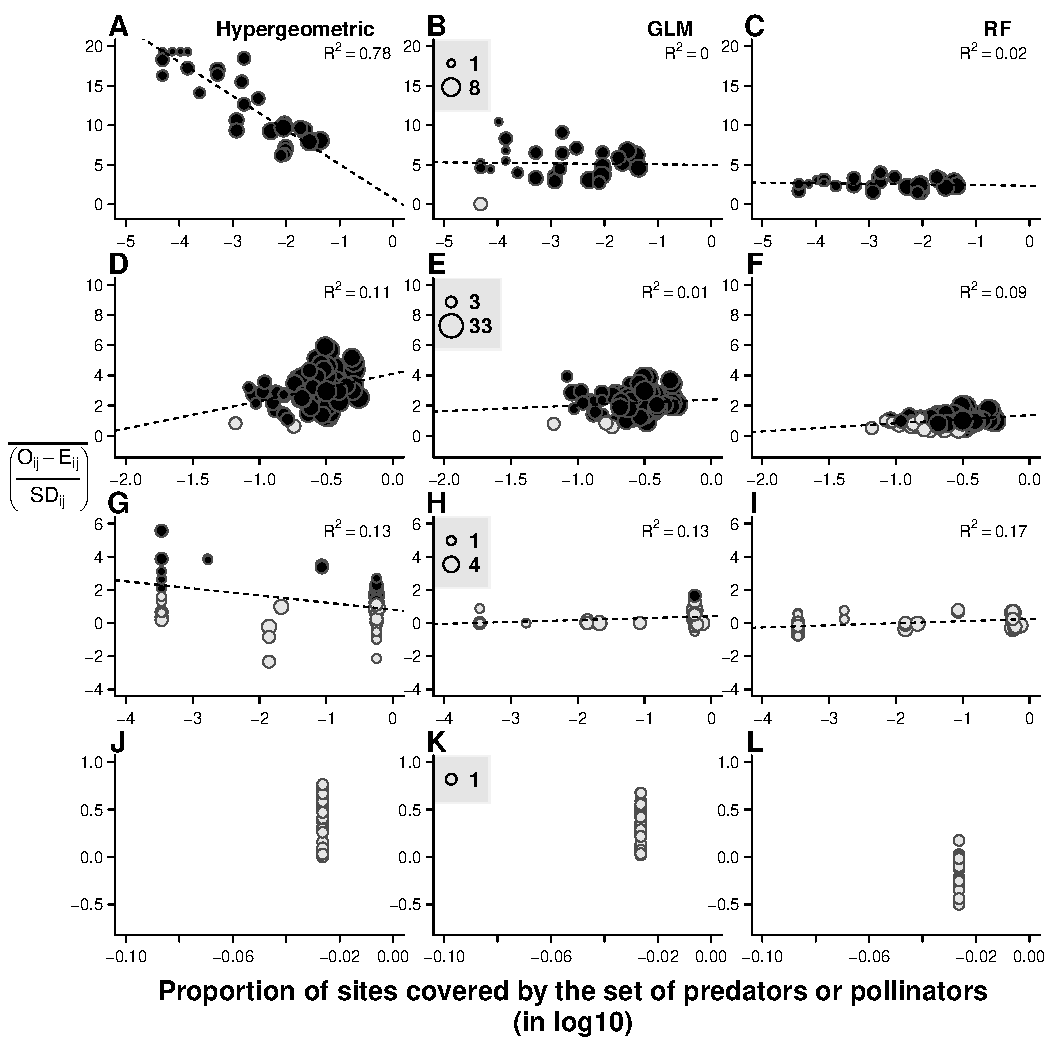
\includegraphics{../fig/figS8.pdf}
\caption{*Reversed figure 4** This figures correspond to the figure 4 in
the main text but the Z-score are calculated for preys (host plants)
rather than for predators 9pollinators). Mean Z-score are computed for
willows (A-C) and herbivores (based on the herbivores-parasitoids only,
D-F) of the willows leafs network, the hosts plants in the Caribbean
hummingbirds datasets (G-I) and species that feed on the detritus in the
pitcher plants network (panels J-L). The x-axis is expressed as a log
proportion of the total number of sites included in the considered
dataset. Black symbols are mean Z-scores significantly different from 0
(see SI Text). In each panel, the dotted line represents the linear
regression \(y~ax+b\) for which the \(R^2\) is provided. The size of
circles reflects the degree of species for which the Z-score was
calculated, the relation size-degree for each row is given in the middle
panel.\label{fig:degocc2}}
\end{figure}

\newpage

\begin{figure}[htbp]
\centering
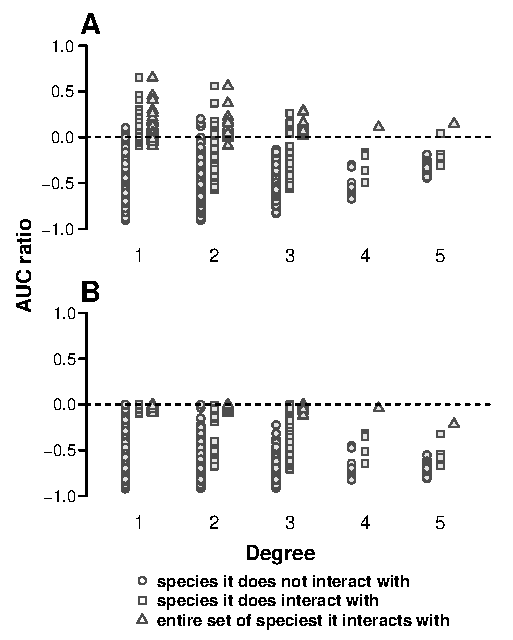
\includegraphics{../fig/figS9.pdf}
\caption{\textbf{Predicting herbivore distribution based on the
distribution of willows} For the herbivores in the willow leafs network
dataset, we compared the AUC obtained when using willow it does not
interact with (circles) a willow in interacts with (squares) and the set
of willow it interacts with (triangles) to AUC obtained for GLM (A) and
RF (B). Positive values indicated that species based model outperformed
the SDM model.\label{fig:ratauc}}
\end{figure}

\newpage

\newpage

\section*{Supporting References}\label{supporting-references}
\addcontentsline{toc}{section}{Supporting References}

\hypertarget{refs}{}
\hypertarget{ref-Dray2007}{}
Dray, S., Dufour, A.B., 2007. The ade4 Package: Implementing the Duality
Diagram for Ecologists. Journal of Statistical Software 22, 1--20.
doi:\href{https://doi.org/10.1.1.177.8850}{10.1.1.177.8850}

\hypertarget{ref-Rcoreteam2015}{}
R Core Team, 2015. R: A Language and Environment for Statistical
Computing.

\hypertarget{ref-Veech2013}{}
Veech, J.A., 2013. A probabilistic model for analysing species
co-occurrence. Global Ecology and Biogeography 22, 252--260.
doi:\href{https://doi.org/10.1111/j.1466-8238.2012.00789.x}{10.1111/j.1466-8238.2012.00789.x}
